\documentclass[a4paper, 14pt]{article}
\usepackage[margin=2.25cm]{geometry}
\usepackage[utf8]{inputenc}
\usepackage{minted}
\usepackage[russian]{babel}
\usepackage{amsmath}
\usepackage{graphicx}
\usepackage{changepage}
\usepackage{hyperref}
\usepackage{cases}
\usepackage{indentfirst}
\usepackage{multirow}
\usepackage{longtable}
\pagestyle{plain}

\hypersetup{
	linkbordercolor = {1 1 1}
}

\usepackage[usenames,dvipsnames,svgnames,table]{xcolor}
\usepackage{tikz-timing}[2009/05/15]
\usepackage{multicol}
\usepackage[T2A]{fontenc}
\usepackage{pgfplots}
\usepackage{pgfgantt}

\usepackage{listings}
\usepackage{caption}
\DeclareCaptionFont{white}{\color{white}} % Текст заголовка.
\DeclareCaptionFormat{listing}{\colorbox{gray}{\parbox{\textwidth}{#1#2#3}}}
\captionsetup[lstlisting]{format=listing,labelfont=white,textfont=white}
\renewcommand\labelenumi{\theenumi)}

\usepackage[backend=biber]{biblatex}
\addbibresource{mybib.bib}

\def\Year{\expandafter\YEAR\the\year}
\def\YEAR#1#2#3#4{#1#2#3#4}



\begin{document}
\lstset{
	language=java,                 % Выбор языка для подсветки (здесь это java).
	basicstyle=\small\sffamily,    % Размер и начертание шрифта для подсветки кода.
	numbers=left,                  % Где поставить нумерацию строк (слева\справа).
	numberstyle=\tiny,             % Размер шрифта для номеров строк.
	stepnumber=1,                  % Размер шага между двумя номерами строк.
	firstnumber=1,
	numberfirstline=true
	numbersep=5pt,                 % Как далеко отстоят номера строк от подсвечиваемого кода.
	backgroundcolor=\color{white}, % Цвет фона подсветки - используем \usepackage{color}.
	showspaces=false,              % Показывать или нет пробелы специальными отступами.
	showstringspaces=false,        % Показывать или нет пробелы в строках.
	showtabs=false,                % Показывать или нет табуляцию в строках.
	frame=single,                  % Рисовать рамку вокруг кода.
	tabsize=2,                     % Размер табуляции по умолчанию равен 2 пробелам.
	captionpos=t,                  % Позиция заголовка вверху [t] или внизу [b].
	breaklines=true,               % Автоматически переносить строки (да\нет).
	breakatwhitespace=false,       % Переносить строки только если есть пробел.
	escapeinside={\%*}{*)}         % Если нужно добавить комментарии в коде.
}

\begin{titlepage}
	\center
	МИНИСТЕРСТВО НАУКИ И ВЫСШЕГО ОБРАЗОВАНИЯ РОССИЙСКОЙ ФЕДЕРАЦИИ\linebreak
	ФЕДЕРАЛЬНОЕ ГОСУДАРСТВЕННОЕ АВТОНОМНОЕ ОБРАЗОВАТЕЛЬНОЕ УЧРЕЖДЕНИЕ ВЫСШЕГО ОБРАЗОВАНИЯ\linebreak
	Национальный исследовательский ядерный университет <<МИФИ>> (НИЯУ МИФИ)
	\noindent\rule{500pt}{0.8pt} \\
	\textsc{\Large Институт интеллектуальных кибернетических систем}\\[8.5cm]

	{ \huge \bfseries ОТЧЕТ ПО ИТОГОВОМУ ПРОЕКТУ	\\
	\Large \mdseries СИСТЕМА УПРАВЛЕНИЯ ЛИЧНЫМИ ФИНАНСАМИ \\
	\large по дисциплине <<Принципы объектно-ориентированного программирования>>}\\[7.0cm]


	\begin{multicols}{2}
		\begin{flushright} \large

			{Выполнил студент группы: М24-535:}\\[0.5cm]

			{Преподаватели:\\}

		\end{flushright}
		\begin{flushright}

			{Почернин В. С.}\\[0.5cm]


			Калин А.\\
			Хлебников А.

		\end{flushright}
	\end{multicols}

	\flushright{
		{\today}\\[0.5cm]
	}
	\centering{
		Санкт-Петербург\\
		\Year
	}

	\vfill
\end{titlepage}

\large
\tableofcontents

\newpage
\section{Описание проекта}

Система управления личными финансами представляет собой приложение, предоставляющее возможность пользователям добавлять доходы и расходы, просматривать статистику по финансам, а также устанавливать бюджеты и категории.

Приложение написано в строгом соответствии с критериями, описанными в \texttt{README.md} (соответствие критериям будет показано ниже).

\subsection{Используемые технологии}

\begin{itemize}
	\item \texttt{Java} - язык программирования.
	\item \texttt{Spring} - основной фреймворк.
	\item \texttt{PostgreSQL} - используемая СУБД.
	\item \texttt{Maven} - система сборки проекта.
	\item \texttt{Flyway} - инструмент для применения файлов миграций БД.
	\item \texttt{Lombok} - библиотека для сокращения шаблонного кода.
\end{itemize}

\subsection{Описание модулей}

Вкратце рассмотрим кодовую базу проекта: \textbf{TODO}.

\begin{itemize}
	\item Пакет \texttt{command}: содержит в себе классы, отвечающие за работу интерфейса командной строки, такие как сама команда, типы команд, а также сам класс интерфейса.
	\item Пакет \texttt{context}: содержит класс, отвечающий за переменные контекста приложения.
	\item Пакет \texttt{entity}: содержит классы моделей данных (связанных с базой при помощи \texttt{ORM}).
	\item Пакет \texttt{exception}: содержит в себе класс-исключение, связанное с системой управления личными финансами.
	\item Пакет \texttt{handler}: содержит в себе классы, реализующие паттерн <<стратегия>> и используемые для обработки команд.
	\item Пакет \texttt{repository}: содержит в себе классы - \texttt{JPA} репозитории.
	\item Пакет \texttt{utils}: содержит в себе различные утильные классы.
	\item Папка \texttt{migration}: содержит в себе файлы миграции БД, которые устанавливают схему и наполняют базу тестовыми данными.
\end{itemize}

\subsection{Схема БД}

База данных проекта имеет следующую схему:

\begin{figure}[H]
	\centering
	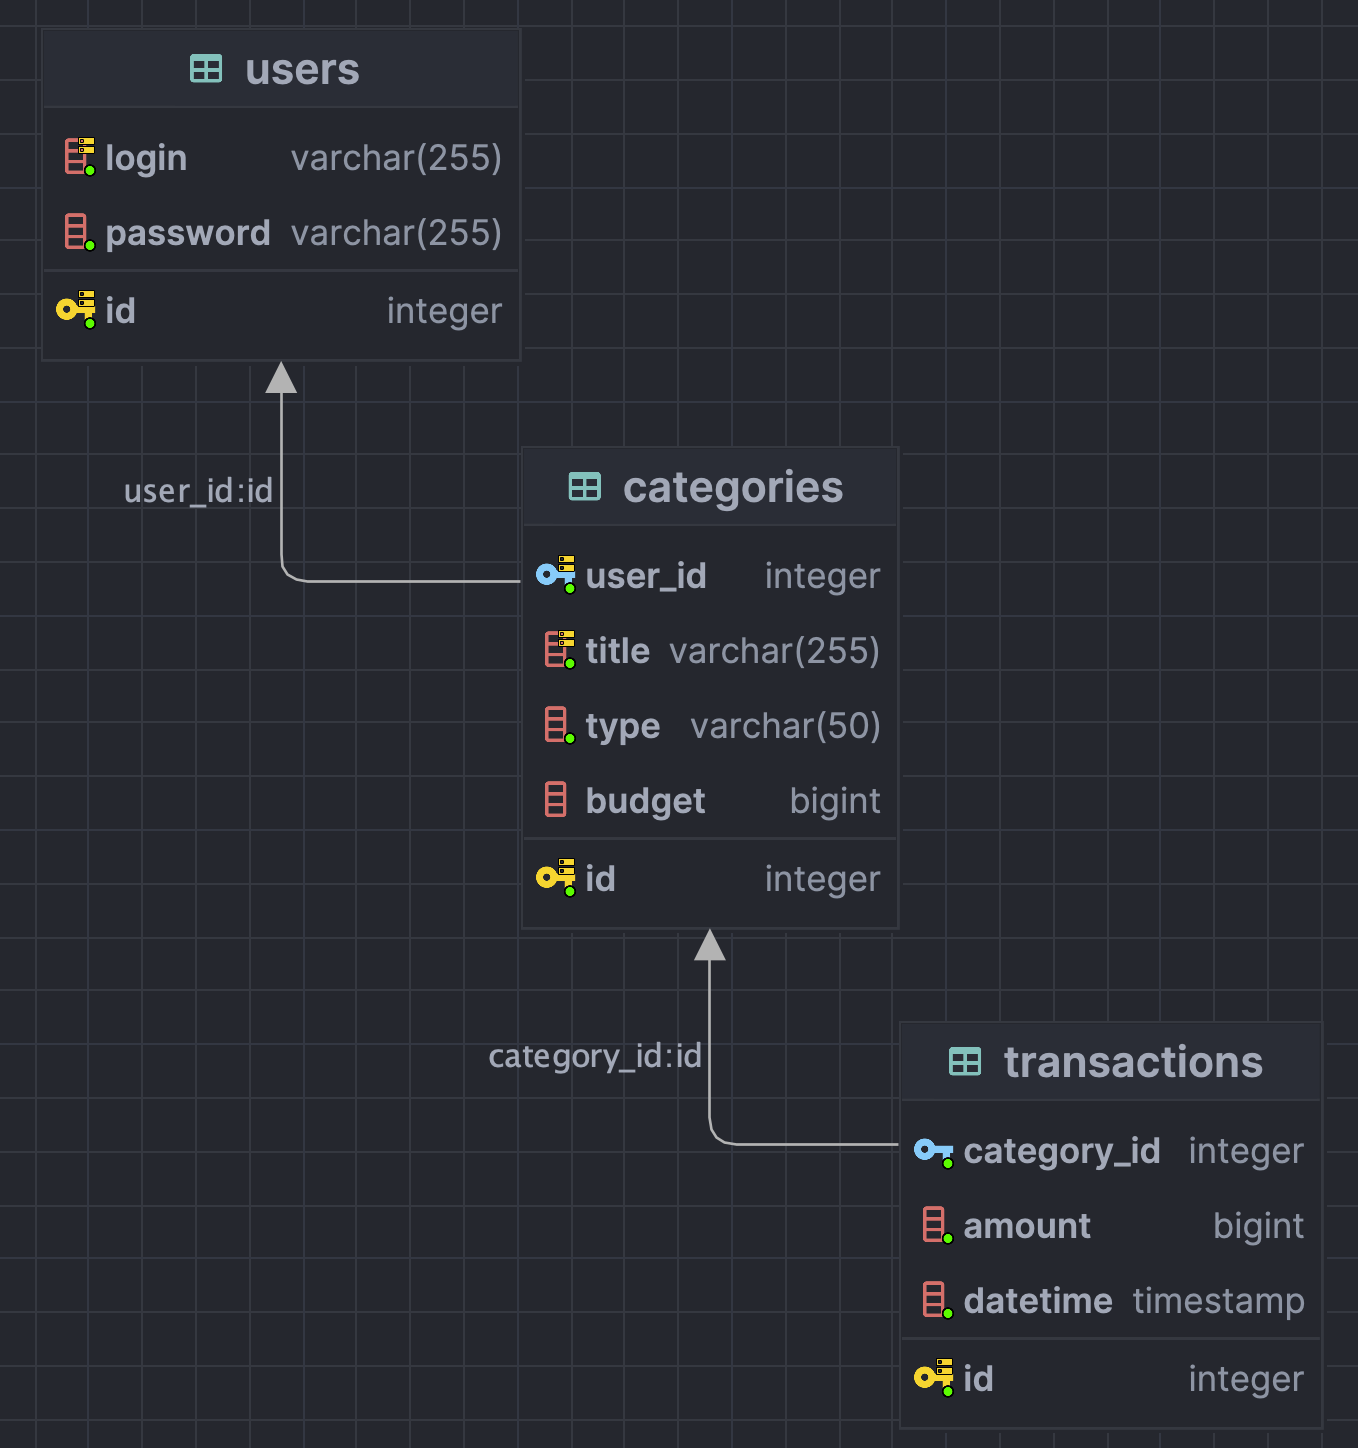
\includegraphics[width=17cm]{resources/1.png}
	\caption{Схема БД}
\end{figure}

\newpage
\section{Инструкции по запуску кода}

Для того, чтобы запустить код, необходимо иметь

\begin{itemize}
	\item \texttt{Java 17} (полагаю, что версии выше также подойдут).
	\item \texttt{Docker} (необходим для быстрого поднятия БД, но можно поднимать руками).
	\item \texttt{Maven} (либо просто запускать проект в \texttt{IntelliJ IDEA}).
\end{itemize}

Запустим наш проект. Для начала, перейдем в директорию, содержащую конфигурационный файл докера - \texttt{/src/main/resources/db}, затем запустим базу данных в \texttt{detach} режиме командой \texttt{docker compose up -d}

\begin{figure}[H]
	\centering
	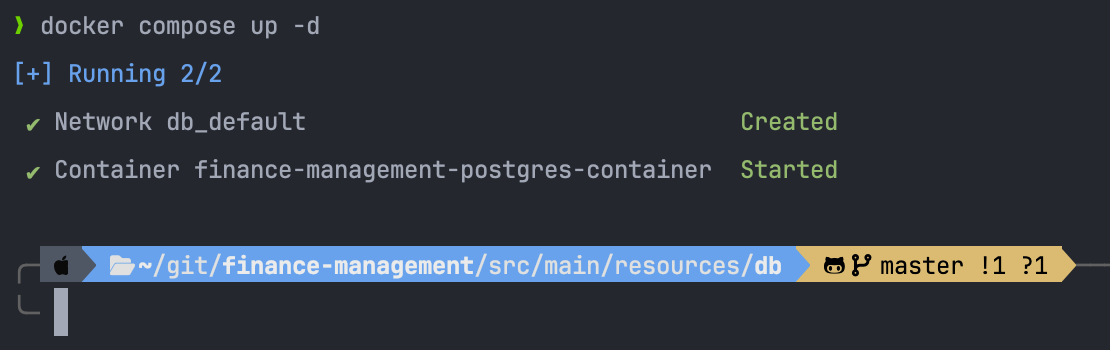
\includegraphics[width=17cm]{resources/2.png}
	\caption{Запуск БД}
\end{figure}

Чтобы собрать проект при использовании \texttt{Maven} вручную, можно написать команду \texttt{mvn clean compile}.

Чтобы запустить сам проект, можно либо сделать это в консоли с помощью \texttt{Maven}, написав команду
\begin{verbatim}
mvn exec:java -Dexec.mainClass=
"ru.vspochernin.short_link_service.ShortLinkServiceApplication"
\end{verbatim}
Либо просто запустить \texttt{main()} метод из класса \texttt{ShortLinkServiceApplication} с помощью \texttt{IntelliJ IDEA} (идея при запуске проекта должна автоматически скачать все зависимости).


После запуска кода, мы увидим приветственное сообщение с описанием всех команд, требованиям к конфигурационному файлу и параметрам.

\textbf{TODO}.

\newpage
\section{Тестирование на соответствие критериям}

Ниже мы пройдемся по каждому критерию и проверим корректность его выполнения.

\textbf{TODO}.

\end{document}